\documentclass[aspectratio=169]{../latex_main/tntbeamer}  % you can pass all options of the beamer class, e.g., 'handout' or 'aspectratio=43'
\usepackage{dsfont}
\usepackage{bm}
\usepackage[english]{babel}
\usepackage[T1]{fontenc}
%\usepackage[utf8]{inputenc}
\usepackage{graphicx}
\graphicspath{ {./figures/} }
\usepackage{algorithm}
\usepackage[ruled,vlined,algo2e,linesnumbered]{algorithm2e}
\usepackage{hyperref}
\usepackage{booktabs}
\usepackage{mathtools}

\usepackage{amsmath,amssymb}

\DeclareMathOperator*{\argmax}{arg\,max}
\DeclareMathOperator*{\argmin}{arg\,min}

\usepackage{amsbsy}
\newcommand{\vect}[1]{\bm{#1}}
%\newcommand{\vect}[1]{\boldsymbol{#1}}

\usepackage{pgfplots}
\pgfplotsset{compat=1.16}
\usepackage{tikz}
\usetikzlibrary{trees} 
\usetikzlibrary{shapes.geometric}
\usetikzlibrary{positioning,shapes,shadows,arrows,calc,mindmap}
\usetikzlibrary{positioning,fadings,through}
\usetikzlibrary{decorations.pathreplacing}
\usetikzlibrary{intersections}
\pgfdeclarelayer{background}
\pgfdeclarelayer{foreground}
\pgfsetlayers{background,main,foreground}
\tikzstyle{activity}=[rectangle, draw=black, rounded corners, text centered, text width=8em]
\tikzstyle{data}=[rectangle, draw=black, text centered, text width=8em]
\tikzstyle{myarrow}=[->, thick, draw=black]

% Define the layers to draw the diagram
\pgfdeclarelayer{background}
\pgfdeclarelayer{foreground}
\pgfsetlayers{background,main,foreground}

% Requires XeLaTeX or LuaLaTeX
%\usepackage{unicode-math}

\usepackage{fontspec}
%\setsansfont{Arial}
\setsansfont{RotisSansSerifStd}[ 
Path=../latex_main/fonts/,
Extension = .otf,
UprightFont = *-Regular,  % or *-Light
BoldFont = *-ExtraBold,  % or *-Bold
ItalicFont = *-Italic
]
\setmonofont{Cascadia Mono}[
Scale=0.8
]

% scale factor adapted; mathrm font added (Benjamin Spitschan @TNT, 2021-06-01)
%\setmathfont[Scale=1.05]{Libertinus Math}
%\setmathrm[Scale=1.05]{Libertinus Math}

% other available math fonts are (not exhaustive)
% Latin Modern Math
% XITS Math
% Libertinus Math
% Asana Math
% Fira Math
% TeX Gyre Pagella Math
% TeX Gyre Bonum Math
% TeX Gyre Schola Math
% TeX Gyre Termes Math

% Literature References
\newcommand{\lit}[2]{\href{#2}{\footnotesize\color{black!60}[#1]}}

%%% Beamer Customization
%----------------------------------------------------------------------
% (Don't) Show sections in frame header. Options: 'sections', 'sections light', empty
\setbeamertemplate{headline}{empty}

% Add header logo for normal frames
\setheaderimage{
	% 
\includegraphics[height=\logoheight]{figures/TNT_darkv4.pdf}
	
\includegraphics[height=\logoheight]{../latex_main/figures/luh_logo_rgb_0_80_155.pdf}
	% 
\includegraphics[height=\logoheight]{figures/logo_tntluh.pdf}
}

% Header logo for title page
\settitleheaderimage{
	% 
\includegraphics[height=\logoheight]{figures/TNT_darkv4.pdf}
	
\includegraphics[height=\logoheight]{../latex_main/figures/luh_logo_rgb_0_80_155.pdf}
	% 
\includegraphics[height=\logoheight]{figures/logo_tntluh.pdf}
}

% Title page: tntdefault 
\setbeamertemplate{title page}[tntdefault]  % or luhstyle
% Add optional title image here
%\addtitlepageimagedefault{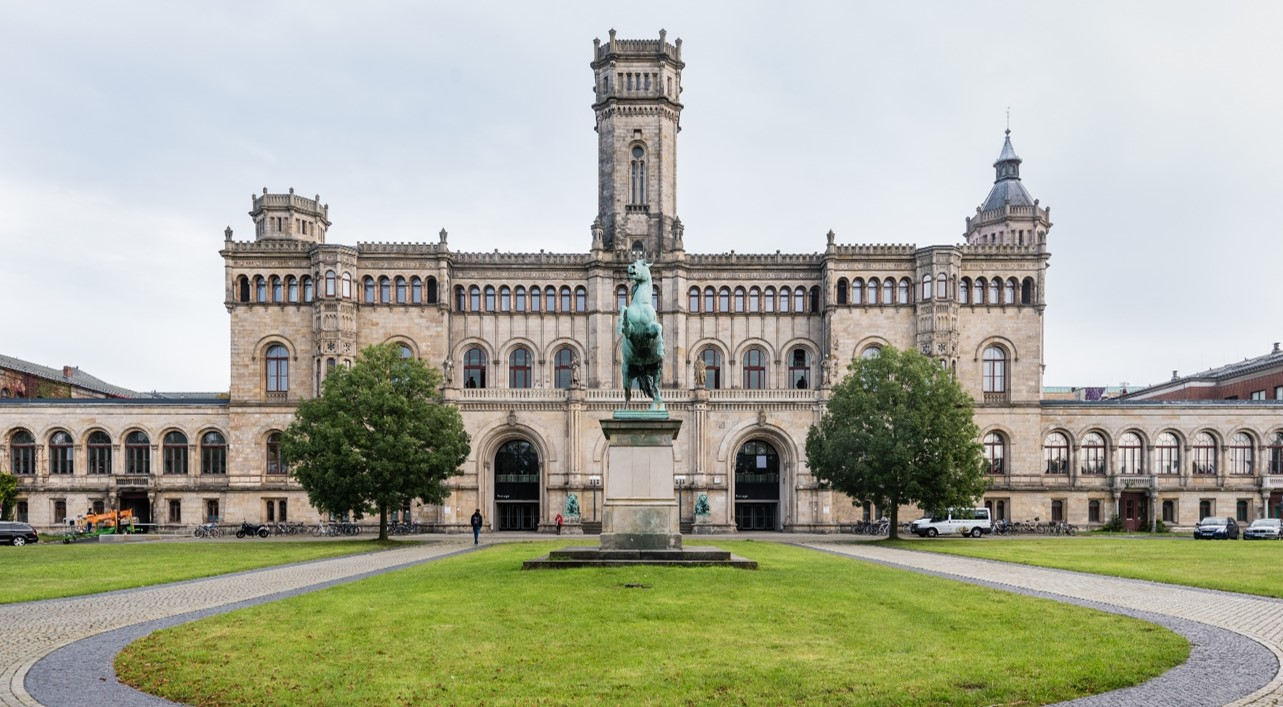
\includegraphics[width=0.65\textwidth]{figures/luh_default_presentation_title_image.jpg}}

% Title page: luhstyle
% \setbeamertemplate{title page}[luhstyle]
% % Add optional title image here
% \addtitlepageimage{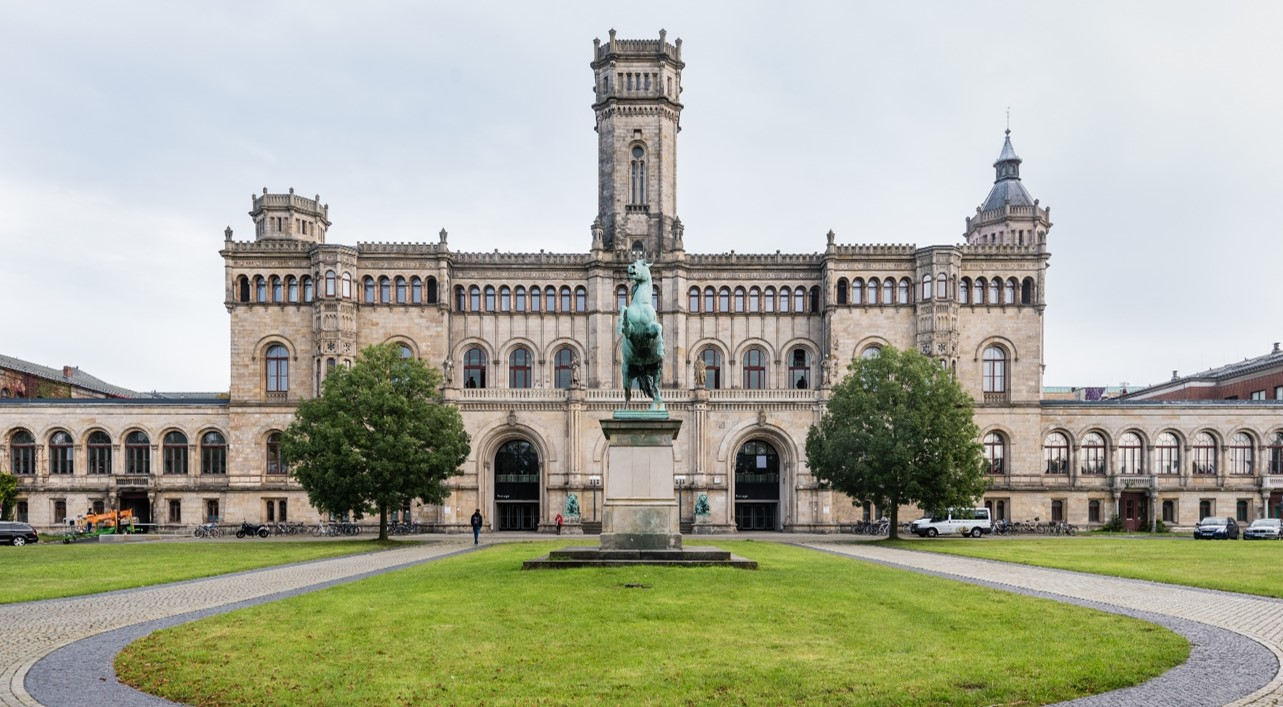
\includegraphics[width=0.75\textwidth]{figures/luh_default_presentation_title_image.jpg}}

\author[Abedjan \& Lindauer]{Ziawasch Abedjan \& Marius Lindauer\\[1em]
	
\includegraphics[height=\logoheight]{../latex_main/figures/luh_logo_rgb_0_80_155.pdf}\qquad
	
\includegraphics[height=\logoheight]{../latex_main/figures/DBIS_Kurzlogo.png}\qquad

\includegraphics[height=\logoheight]{../latex_main/figures/TNT_darkv4}\qquad

\includegraphics[height=\logoheight]{../latex_main/figures/L3S.jpg}	}
\date{Summer Term 2022; \hspace{0.5em} {
\includegraphics[height=1.5em]{../latex_main/figures/Cc-by-nc-sa_icon.svg.png}}; based on \href{https://ds100.org/fa21/}{[DS100]}
}


%%% Custom Packages
%----------------------------------------------------------------------
% Create dummy content
\usepackage{blindtext}

% Adds a frame with the current page layout. Just call \layout inside of a frame.
\usepackage{layout}


%%% Macros
%\renewcommand{\vec}[1]{\mathbf{#1}}
% \usepackage{bm}
%\let\vecb\bm

\title[Introduction]{DS: Clustering, Part 2}
\subtitle{Affinity Matrices}

\graphicspath{ {./figure/} }
%\institute{}


\begin{document}
	
	\maketitle
	\begin{frame}{Creating a Graph from Point Data}
	    It turns out that spectral clustering methods work really well on some types of traditional Euclidean point datasets (design matrices).\\
	    \bigskip
	    To use spectral clustering on a basic design matrix, we construct a graph from our data. This is actually the default setting in scikit-learn’s SpectralClustering method.\\
	    \bigskip
	    Each individual row in our design matrix will become a vertex in our new graph, and the edges between them represent how “close,” or how “related” each pair of points is.\\
	    \bigskip
	    There are two common ways of creating such graphs, we will discuss both.
	\end{frame}
	
	
	\begin{frame}{Example Dataset}
	    Let’s say we have a dataset with 4 individuals and 2 features, like so:
	    \begin{figure}
	        \centering
	        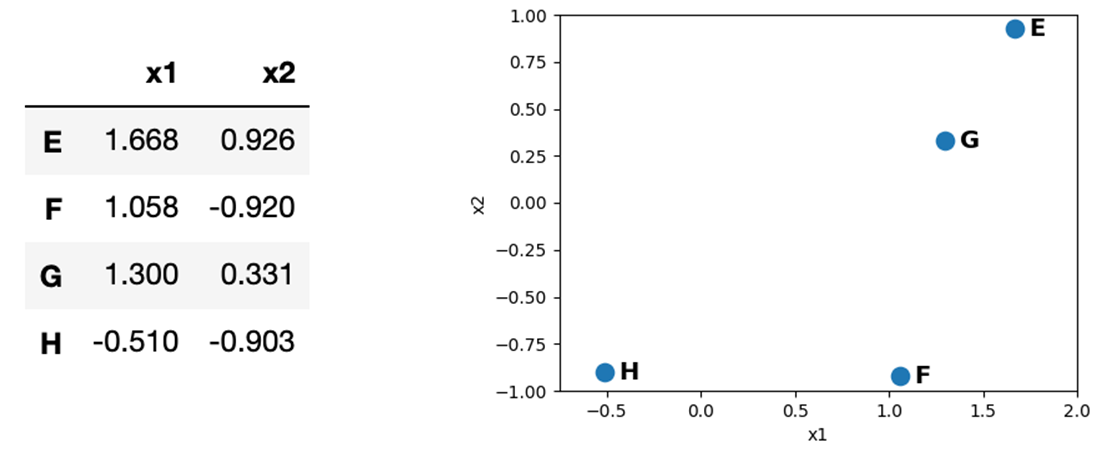
\includegraphics[scale=.5]{Bild17}
	    \end{figure}
	\end{frame}
	
	
	\begin{frame}{Points to Graph Method \#1: Distance Matrix}
	    One way to construct a graph based on data is to have the edges be some measure of the distance\\ between each pair of points.\\
        To do so, we can calculate the distance matrix.

	    \begin{figure}
	        \centering
	        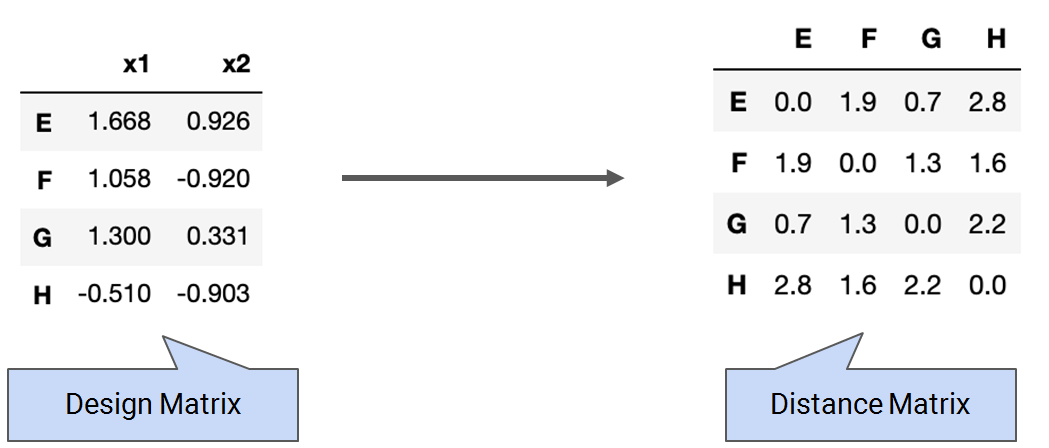
\includegraphics[scale=.4]{Bild18}
	    \end{figure}
	\end{frame}
	
	
	
	\begin{frame}{Question}
	    Q: Should the weight of an edge between two vertices be equal to the distance between the two corresponding points?\\
	    \bigskip
	    A: No! Larger edge weights should indicate a stronger relationship between two vertices, but a large distance between two parts means they are far apart, and do not have that strong of a relationship.

	\end{frame}
	
	
	\begin{frame}{Points to Graph Method \#1: Distance Matrix}
	    To determine the edge weights, we apply a decaying function to the distance matrix.\\
        Now, larger distances will lead to smaller edge weights, and vice versa.\\
        Common choice:       $e^{-\gamma d}$        , where d is the distance, and $\gamma$ is some chosen constant.

        \begin{figure}
            \centering
            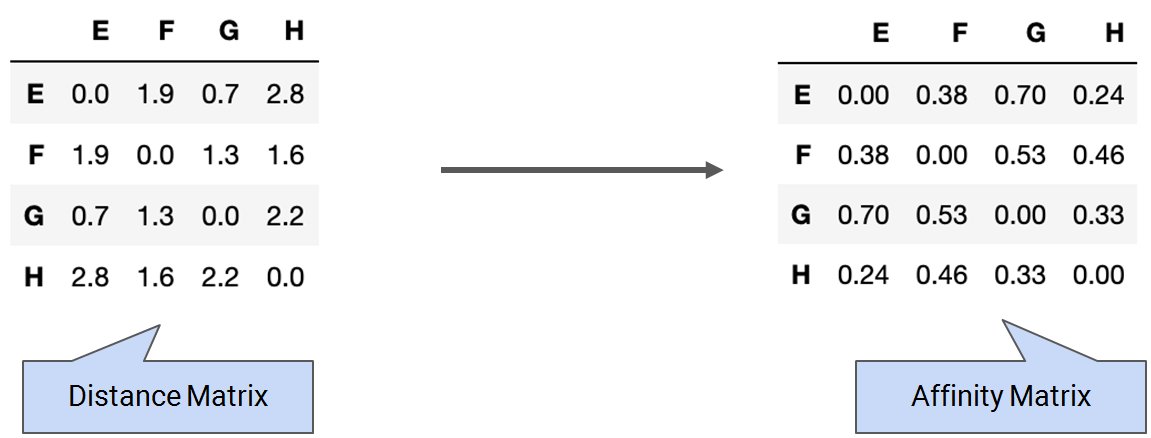
\includegraphics[scale=.43]{Bild19}
        \end{figure}    
	\end{frame}
	
	
	
	\begin{frame}{Points to Graph Method \#1: Distance Matrix}
	    Here is the resulting graph:
	    \begin{figure}
	        \centering
	        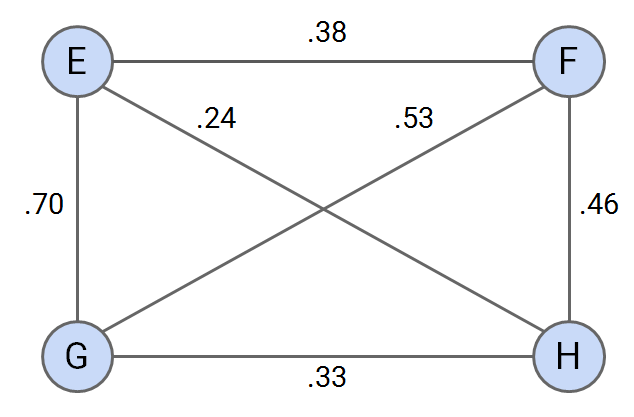
\includegraphics[scale=.5]{Bild20}
	    \end{figure}
	\end{frame}
	
	
	\begin{frame}{Points to Graph Method \#2: Nearest Neighbors}
	    The other way to construct a graph is two draw an edge between points i and j, if j is one of\\ the \_\_ nearest neighbors of i. You choose \_\_\\
        Example, with 1 nearest neighbor:
	    \begin{figure}
	        \centering
	        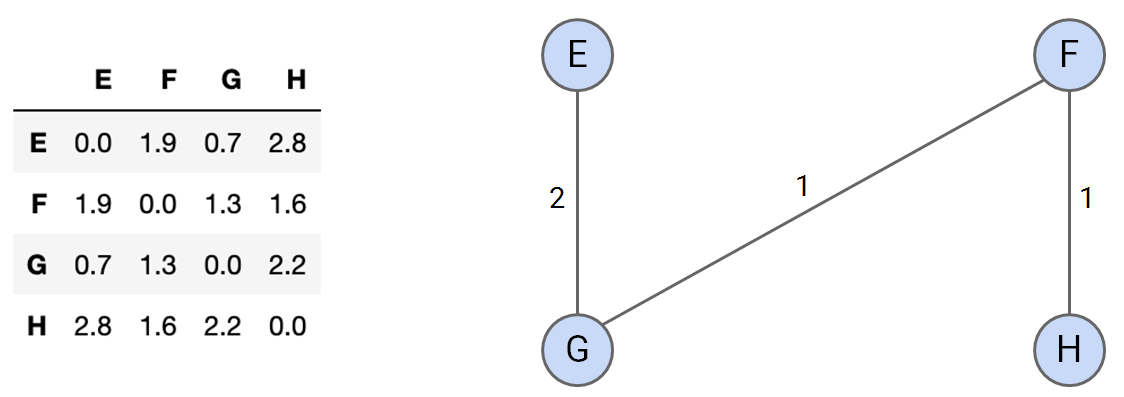
\includegraphics[scale=.48]{Bild21}
	    \end{figure}
	\end{frame}
	
	
	
	\begin{frame}{Recap}
	    If we are given point data (not a graph), we can still use spectral methods to cluster the points.\\
	    \bigskip
	    To do so, we construct a graph from the points, using either a function of the distance matrix, or nearest neighbors.\\
	    \bigskip
	    Usually, we don’t care about the actual graph, only the adjacency matrix.
	    \begin{itemize}
	        \item Such matrices are often also called “affinity matrices,” because they describe the strength of the relationship between the points.
	    \end{itemize}
	    \bigskip
	    Which method you choose is dependent on your application—if you’re stuck, try both!
	\end{frame}
\end{document}